\subsection{Linear equations}
	In our model a node is connected to 4 tubes, or less if the node is located at the edges or a corner. The two-dimensional model can be extended to a three-dimensional case similar to \cite{sinha2017effective}.
	
	When generating the linear equations. For each row it is necessary to do the following for each direction:
	
	\[ [P_i] += R_{ij}K_{ij} \]
	\[ [P_j] -= R_{ij}K_{ij} \]
	\[ [const] -= 2s_{ij}\sigma K_{ij} \]
	
	Here let $K_{ij} = R^3_{ij}/{M}_{ij}$.

	For simplicity we rewrite the system of four euqations as ... [UNDER Construction]
	
	
	In case of 5 nodes in our system, where the pressure of the bottom and top nodes are given and fixed, the matrix for Gaussian elimination will be:

	\[ 
	\begin{pmatrix}
		1 & 0 & 0 & 0 & 0 & P_{up}\\
		0 & 1 & 0 & 0 & 0 & P_{up}\\
		-R_{31}K_{31} & -R_{32}K_{32} & (R_{3k}K_{3k} + ...) & -R_{34}K_{34} & -R_{35}K_{35} & -2\sigma(s_{3k}K_{3k} + ...)\\
		0 & 0 & 0 & 1 & 0 & P_{down}\\
		0 & 0 & 0 & 0 & 1 & P_{down}
	\end{pmatrix}
	\]
	 It can be proven that this matrix always has a solution. Once the solution is determined the flow rate can be calculated using equation \ref{eq:flow-rate-main}, and the velocity of flow in each tube is given by
	 
	\begin{equation} \label{eq:velocity-in-tube}
		\boxed{v_{ij} = \frac{R_{ij}}{8lM_{ij}}(R_{ij}\Delta P_{ij} + 2s_{ij}\sigma)}
	\end{equation}
	
	
\subsection{Numbering tubes and other parameters in the network model}

	\begin{figure}[H]
		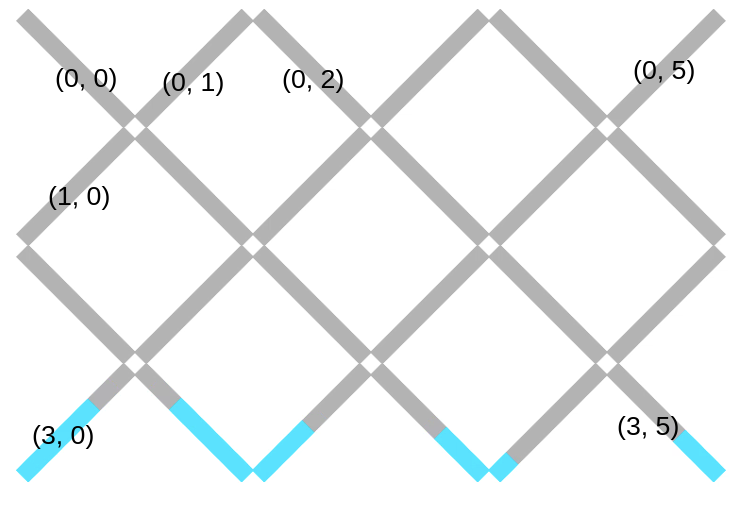
\includegraphics[height=6cm]{fig_numbering-of-ij-tube}
		\caption{Numbering of tubes for a (rows, cols) = (4, 6) network model}
		\label{fig_numbering-of-ij-tube}
	\end{figure}
	
	If $X$ is a parameter then $X_{ij}$ is on the $i$ th row and $j$ th column, note that counting begins from zero. This type of counting is suitable for std::vector< data structure in C++. 
	
\subsection{Solution of Linear Equations}

	\subsubsection{Case of zreo row}
	When we solve the system of linear equations, more than one row can be zeros.

	This problem rarely occurs when there is a larger pressure difference between the top and bottom row of nodes. Rarely because it is possible to have a subsystem even when there is a significant pressure difference between the top and bottom nodes, where the system of linear equations have infinitely many solutions. 


	\subsubsection{Initial configuration for flow to start}

	The flow did not start when all the meniscus were located inside the nodes. Because in our model we assumed that there is not capillary pressure in the nodes. To overcome this, the meniscus were made to be situated inside the tubes.

	\subsubsection{Case of all meniscus located in the thick tubes}

	The solution of linear equation were such that, the capillary force balanced out the pressure gradient. The pressure was much higher outside in the thick tubes than in the thin tubes. Whether this was caused by error in the process of solving the linear equation or due to the initial setup, needs to be checked again. Error is, that it is impossible to determine whether the coefficient during the process of gauss elimination is zero or not. Because of the way how floating point numbers are handled by the CPU, 0 is often seen as a small number.

\subsection{Description of the Model}
	The algorithms and methods used to simulate two-phase flow in porous media has many practical applications in oil recovery, hydrology, electricity production where pressurized water is passed through heated pipes and is transformed into steam, etc. Our algorithm presented here is used to find the saturation of a phase with respect to time, the hysteresis curve when the pressure across the porous body is reversed, total capillary pressure as a function of saturation[4], and determination of permeability which appears in Darcy’s law.

	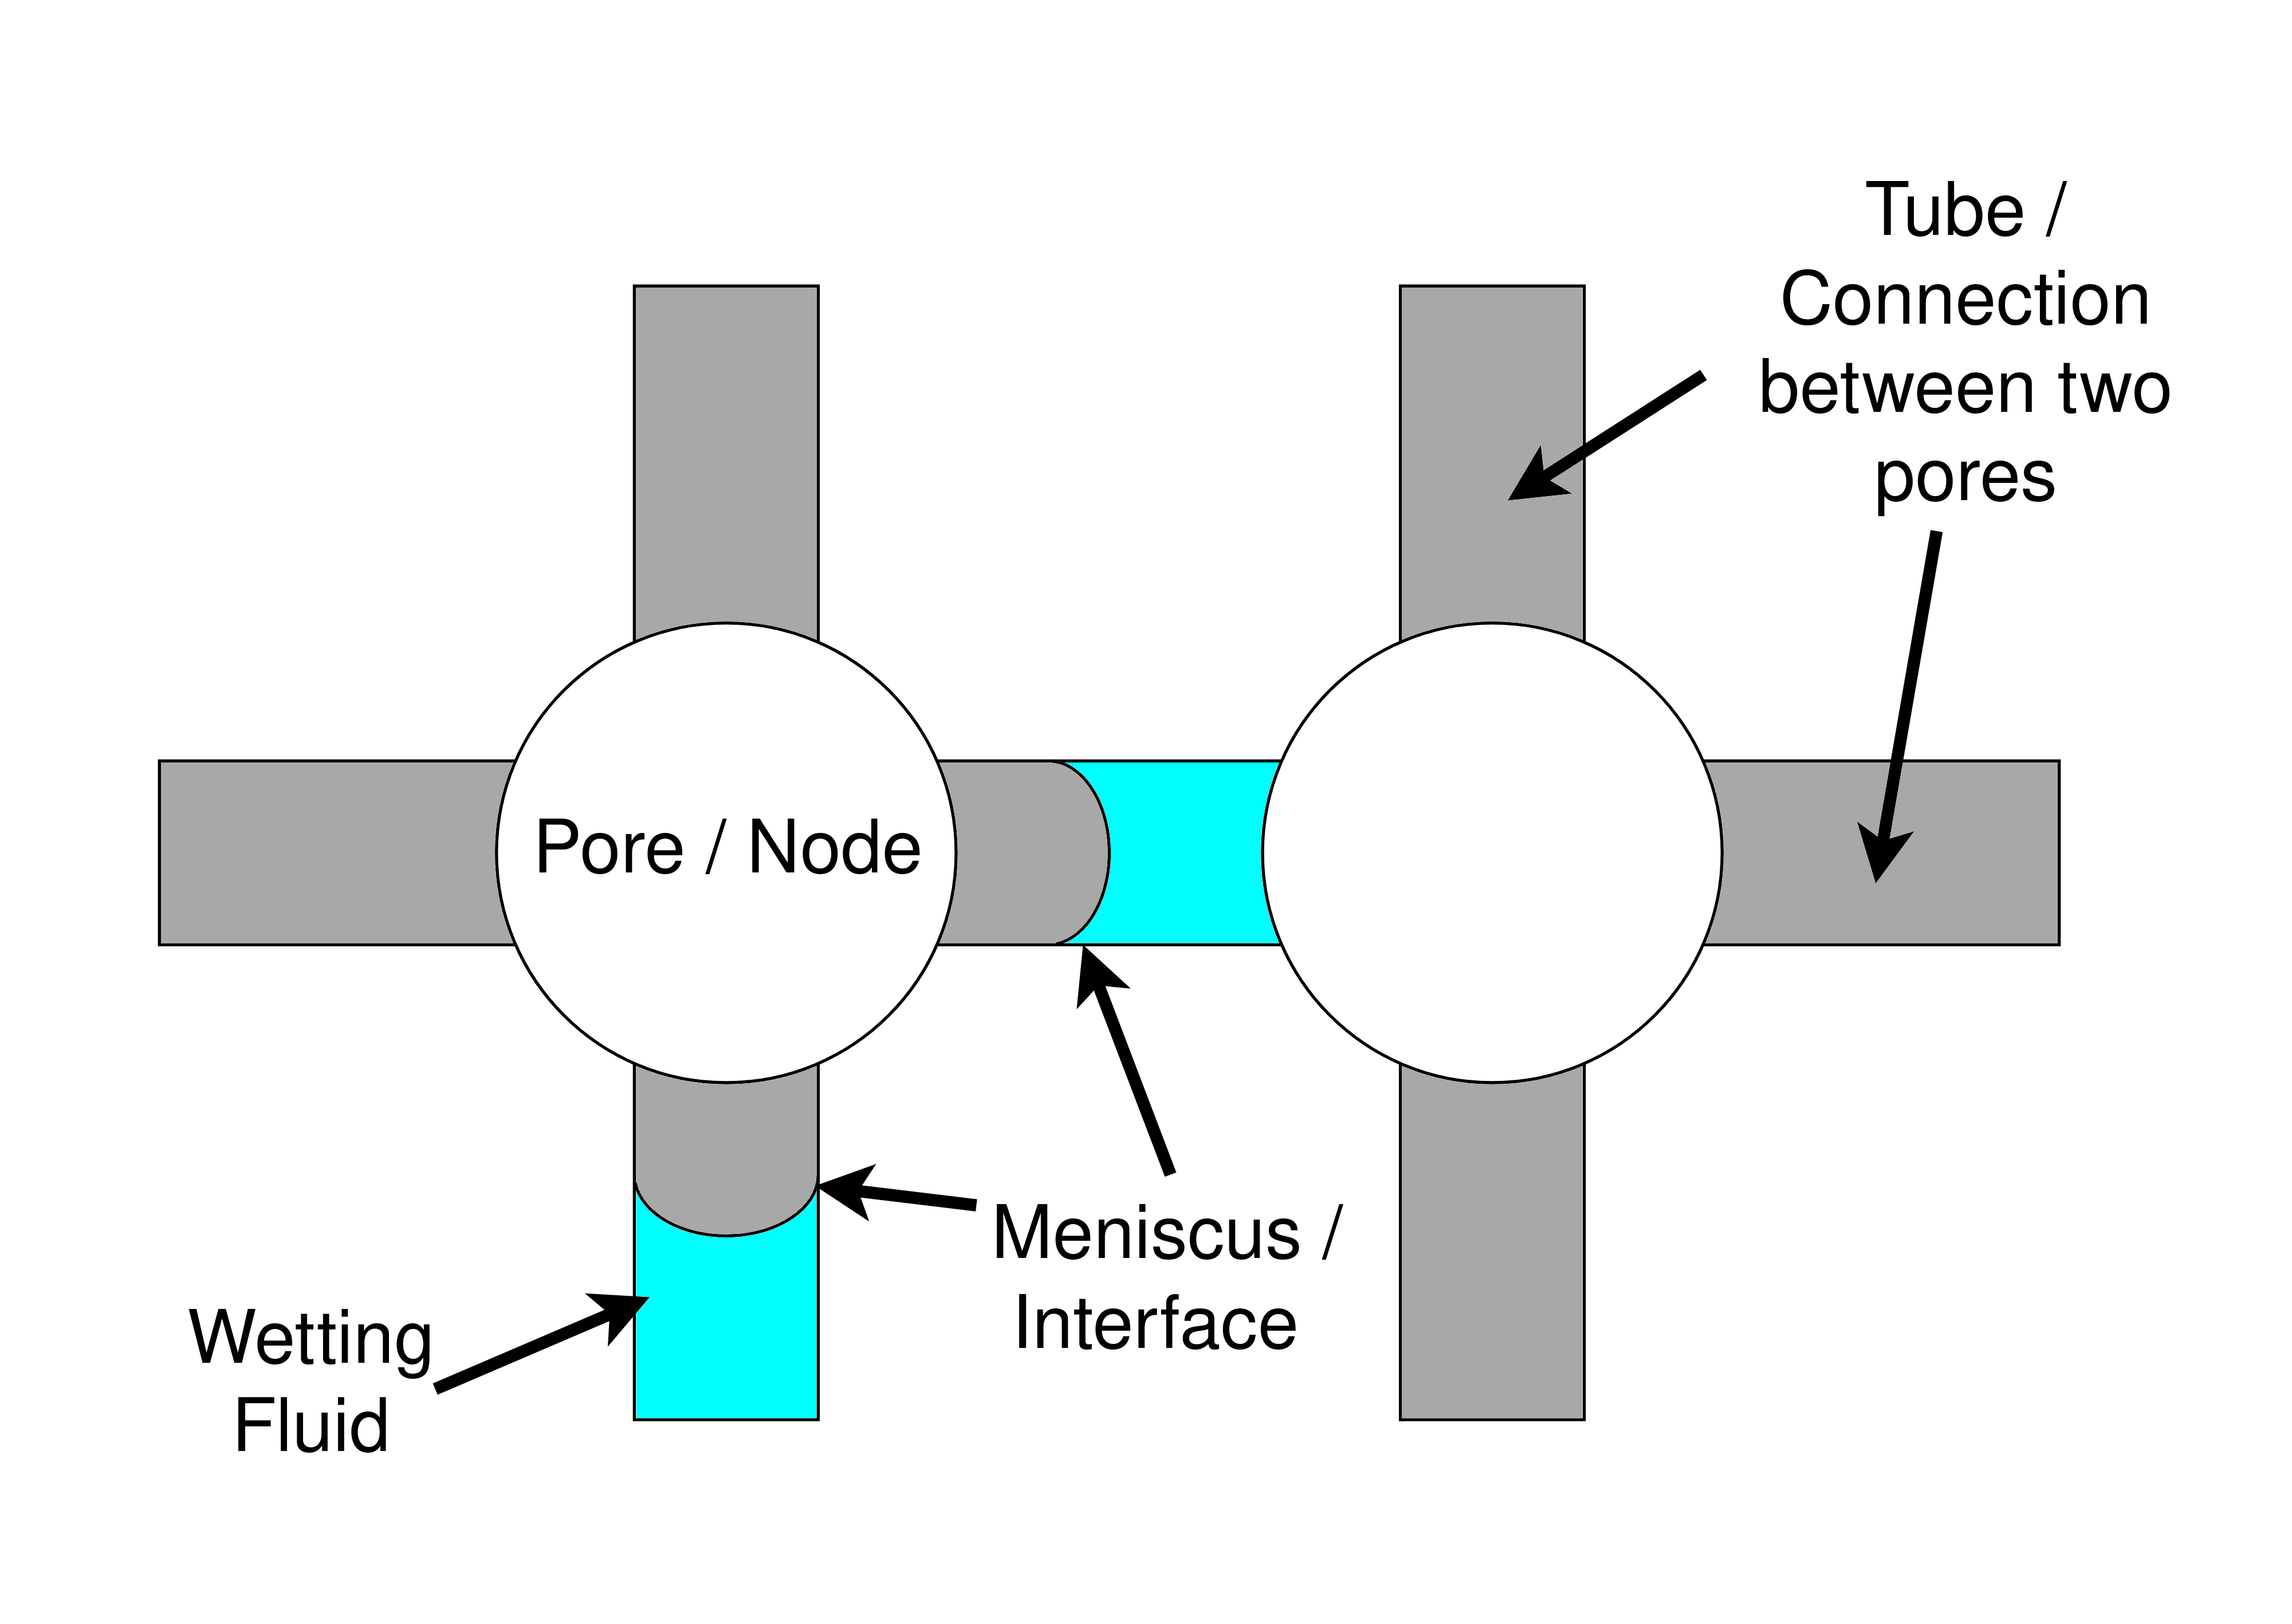
\includegraphics[height=6cm]{fig_descp-of-model}
	
	Figure showing two nodes from the network where the size of the node is much larger than the radius such that the capillary force tends to zero when the meniscus enters a node. 

\subsection{Algorithm for computation}
	\begin{enumerate}
		\item \textbf{Input Files:} read input files, radius.txt and mns.txt, mns.txt contains the initial setup of the meniscus
		\item \textbf{Random radius:} add very small random values to the radius, this is done in order to remove the case of two equal radius for simplicity, can be removed later
		\item \textbf{Loop time:} do until a certain proportion of invading fluid is reached for example 0.90 or a fixed number of frames:
		
		\begin{enumerate}
			\item \textbf{Pressure:} determine the pressure at each node using the linear equations given in section \ref{sec:linear-equ}.
			\item \textbf{Velocity:} Calculate the velocity using equation \ref{eq:velocity-in-tube} 
			\item \textbf{time step:} determine the time step, it is the $\Delta t = min{l/v{i}}$.
			\item \textbf{volume:} The volume displaced in each tube is determined by iterating through all the tubes, $V_{ij} = v_{ij} * t_{min}$.
			\item \textbf{integration:} 
				\begin{enumerate}
				\item \textbf{Store insertion:} create a matrix to store how much of which fluid to insert in each of these tubes.
				\item \textbf{Loop nodes:} Iterate through all the nodes, and for each of the nodes. 
					\begin{enumerate}
						\item divide the tubes into two categories, flow-in-tube - here the fluid from these tubes flow into the nodes, flow-out-tubes here we insert the fluid into the tube from the node
						\item Find out the total of fluid1, fluid2, which is the total of each fliud from all flow-in-tubes.
						\item Start filling the each of the flow-out-tubes where the flow will go into in ascending order of the radius of the tube. This will be done simply be adding the quantity of fluid1 and fluid2 to the matrix created above.
						\item while filling fist use fluid1, once fluid1 is used up then start using fluid2, which means if in a tube we have to insert two fluids, then fluid1 will go in first.
					\end{enumerate}
				\item \textbf{Fluid addition:} For each of the tubes, add the volume of fluid determined to be added. After addition if there are more than 2 meniscus, then merge them retaining their center of masses.
				\end{enumerate}
			\item \textbf{Picture:} Save a picture of the current configuration.
			\end{enumerate}
		\item {Video:} Make a video file from the pictures.
	\end{enumerate}
